% Propiedades del documento
\documentclass[12pt]{report}

\usepackage[spanish,es-tabla]{babel}
\usepackage[utf8]{inputenc}
\usepackage[section]{placeins}
\usepackage{titlesec}
\usepackage{color}
\usepackage{graphicx}
\usepackage[a4paper,width=150mm,top=25mm,bottom=25mm,bindingoffset=6mm]{geometry}
\usepackage{fancyhdr}
\pagestyle{fancy}
\usepackage{subfig}

\usepackage{hyperref}

% Estilo de los enlaces
\hypersetup{
    colorlinks=true, % make the links colored
    linkcolor=black, % color TOC links in blue
    urlcolor=blue, % color URLs in red
    linktoc=all % 'all' will create links for everything in the TOC
}

\setlength{\headheight}{15pt}

% Quitar texto "Capítulo N"
\titleformat{\chapter}[hang]{\Huge\bfseries}{\thechapter{. }}{0pt}{\Huge\bfseries}

% Encabezado y pie de página
\fancyhead{}
\fancyhead[R]{Robot con pasillos estrechos}
\fancyfoot{}
\fancyfoot[R]{\thepage}
\fancyfoot[L]{Costel Adi Huzum \\ Andriy Byelikov \\ Eloy Tolosa Gómez}
\renewcommand{\headrulewidth}{0.4pt}
\renewcommand{\footrulewidth}{0.4pt}

% Color de los títulos
\titleformat{\chapter}{\color{red}\large}{}{0em}{\MakeUppercase}[\titlerule]

% Imágenes
\graphicspath{ {images/} }

\begin{document}

% Portada
\begin{titlepage}
    \begin{center}
 
        %\vfill
 
        %\vspace{0.8cm}
 
        
\includegraphics[width=0.4\textwidth]{logo}
        
        \vspace*{1cm}
 
        \vspace{0.5cm}
 
        \vspace{1.5cm}
        
        \Huge
        \textbf{La cueva del monstruo}
        
        \vfill
 
        \Large
        
        \textbf{Sistemas Inteligentes}\\
        
        \vspace{1.5cm}
        
        Costel Adi Huzum\\
        Andriy Byelikov\\
        Eloy Tolosa Gómez

    \end{center}
\end{titlepage}

 % Índice
\tableofcontents

% Capítulos
\chapter{Enunciado}
La práctica consiste en implementar el problema del robot que recorre el perímetro de un objeto, pero se permite la existencia de pasillos estrechos. En este caso, el robot debe ser capaz de recorrer estos pasillos sin que afecte a su recorrido. Además, en el caso de que el pasillo se encuentre bloqueado, el agente debe recorrerlo hasta al final, dar la vuelta y volver a recorrer el pasillo hasta la entrada de éste.

Finalmente, hay que implementar un interfaz agradable que permite la creación de objetos en una cuadrícula arbitraria y poner al robot en cualquier posición de la cuadrícula.

\begin{figure}[!ht]
    \centering
    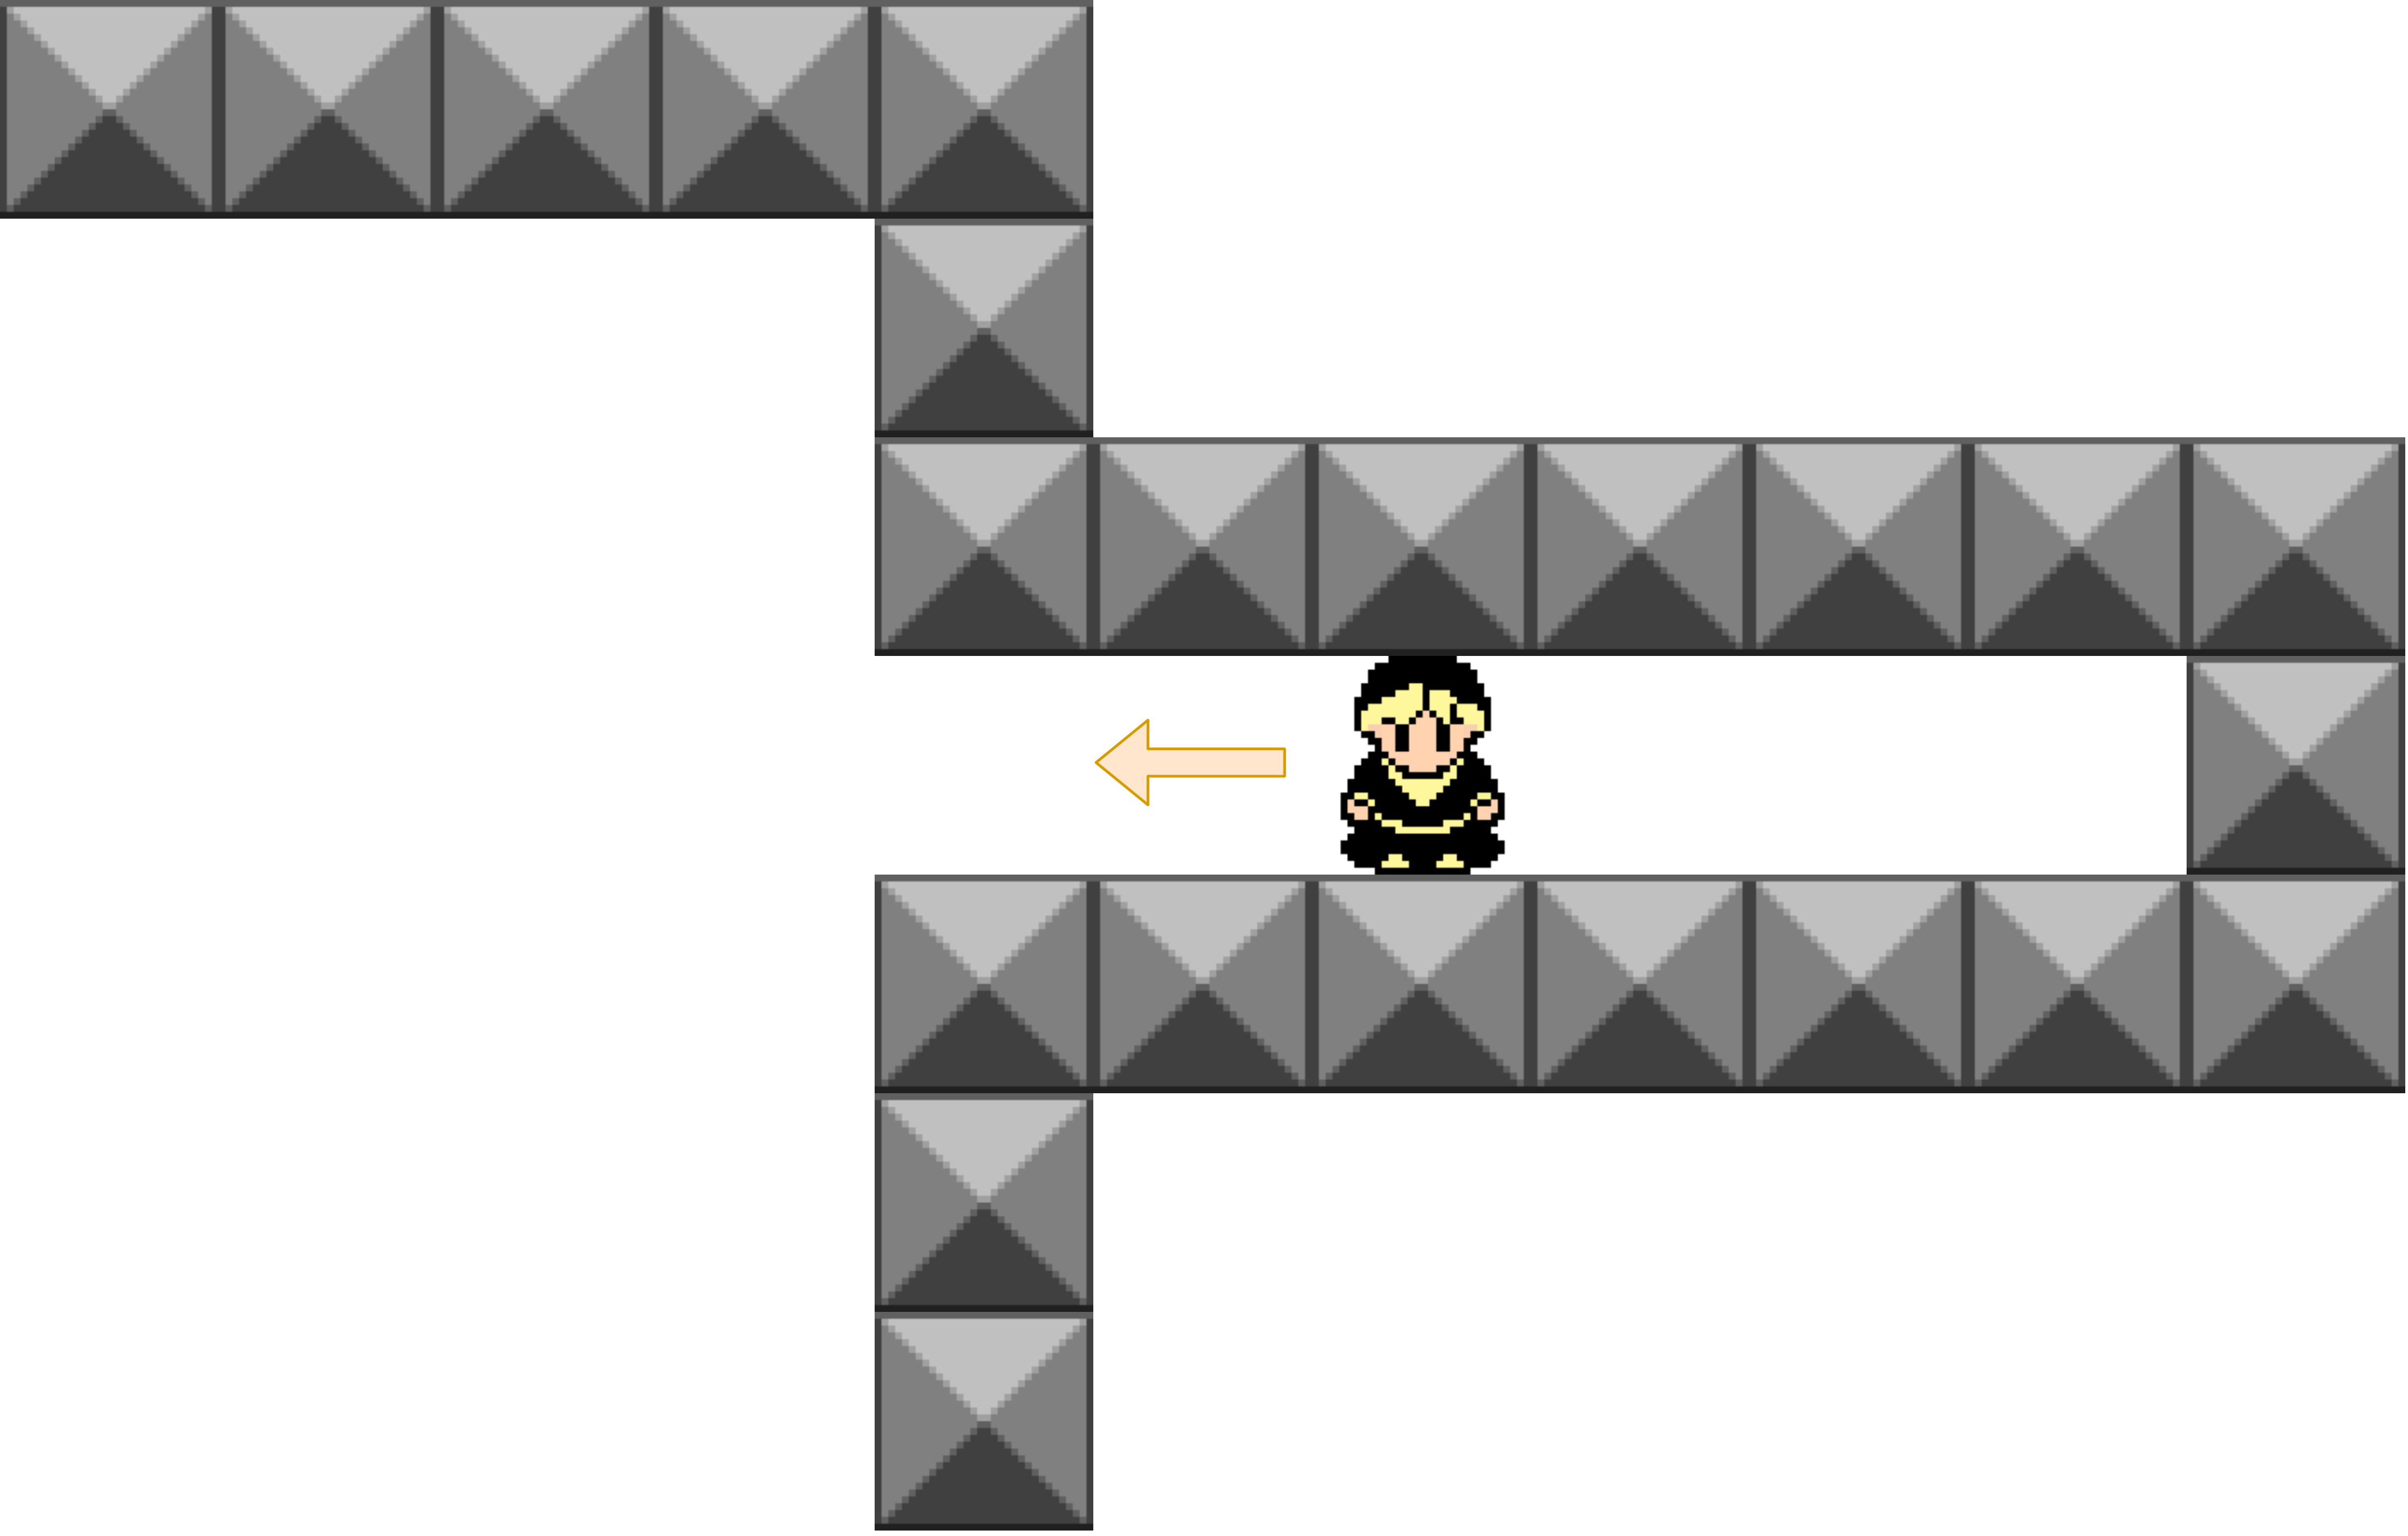
\includegraphics[width=1\textwidth]{example}
    \caption{Ejemplo de pasillo estrecho}
    \label{fig:ejemplo}
\end{figure}

\chapter{Entorno}
El entorno es la base inicial del conocimiento del agente, es de donde el agente recibe las percepciones a partir de las cuales puede formar su vector de características. En este caso en concreto, nuestro entorno va a ser dinámico ya que los diferentes elementos del mismo puede ir cambiando: por ejemplo, el agente puede matar un monstruo y puede poner bombas de hedor para confundir a los otros agentes, lo cual puede hacer que momentáneamente cambie el entorno de otro agente.

El entorno se compone de un mapa de elementos (\emph{Monstruo}, \emph{Precipicio}, \emph{Tesoro}, \emph{Muro} y \emph{Hedor}), un número de agentes, monstruos y tesoros (determinado por el usuario). Éstos elementos los separaremos en dos tipos: Elementos \textbf{estáticos} y elementos \textbf{dinámicos}.
\begin{itemize}
    \item Los elementos \textbf{estáticos} serán los elementos que permanezcan inalterables en el entorno durante la duración del programa. En nuestro caso serán:
    \begin{enumerate}
        \item Paredes.
        \item Precipicios.
    \end{enumerate}
    \item Los elementos \textbf{dinámicos} serán los elementos que podrán cambiar de estado y/o posición durante la duración de la ejecución del programa. Serán:
    \begin{enumerate}
        \item Monstruos (y los hedores que produce).
        \item Las bombas de hedor.
        \item Los tesoros (y su resplandor).
    \end{enumerate}{}
\end{itemize}{}

En esta práctica, nuestro agente se supone que es ciego: esto es, que no puede ver lo que tiene alrededor de él, simulando que está en una cueva oscura y no puede ver lo que hay cerca suya. Por tanto, para que el agente pueda inferir conocimiento, el entorno tendrá que enviarle percepciones. Estas percepciones serán distintas dependiendo de los elementos que haya en el entorno en un momento en concreto. 
Las percepciones que puede enviar el entorno al agente son las siguientes:
\begin{enumerate}
    \item Cuando, en una casilla en concreto, haya un monstruo, éste desprende un \textbf{hedor} que el agente podrá percibir si está en una casilla colindante a la posición del monstruo. \footnote{Una casilla colindante a otra es una casilla que está justo a su lado, a cualquiera de los lados menos en casillas diagonales a la misma.}
    \item Cuando, en una casilla en concreto, haya un precipicio, el agente percibirá una \textbf{brisa} que, de la misma manera que la percepción anterior, el agente percibirá cuando esté en una casilla colindante al precipicio.
    \item Cuando el agente esté situado en la misma casilla donde se encuentre el tesoro, éste emitirá un \textbf{resplandor} que el agente percibirá para poder coger el tesoro. Por cuestiones de completitud, tendremos que forzar que el tesoro no se encuentre en la misma casilla que un precipicio ni un monstruo, ya que, si no, para el agente sería imposible llegar a encontrar el tesoro nunca.
    \item Como extensión de nuestra práctica, cada agente podrá tirar bombas fétidas por el entorno con tal de confundir a los otros agentes y poder conseguir la mayor cantidad de tesoros posibles. Esta bomba fétida emitirá, de la misma manera que el monstruo, un \textbf{hedor}, que permanecerá durante un tiempo determinado y luego se irá, que el agente percibirá cuando se encuentre en la misma casilla en la que se sitúa la bomba fétida.
    \item Cuando un agente tira una flecha a un monstruo y lo mata, éste emite un \textbf{gemido} que es percibido por el agente.
\end{enumerate}{}

Para enviar las percepciones, el entorno sigue el siguiente proceso por cada agente:

\begin{enumerate}
    \item Obtiene la posición del agente.
    \item Obtiene la acción anterior del agente (la que ha realizado en el ciclo anterior).
    \item Si el agente quiere recoger un tesoro que ha encontrado, comprobar que sea un tesoro, quitarlo del mapa e incrementar el número de tesoros encontrados en el mapa.
    \item Preparar las percepciones que se enviarán al agente:
    \begin{enumerate}
        \item Si el agente ha disparado, comprobar si impacta con un \emph{Monstruo}. En caso de que impacte, eliminar el monstruo del mapa y preparar la percepción de \emph{Gemido} (poner su valor a \emph{Verdadero}).
        \item Si se encuentra en la casilla adyacente a un \emph{Monstruo} o en una casilla con \emph{Hedor falso}, preparar la percepción de \emph{Hedor}.
        \item Si se encuentra en la casilla adyacente a un \emph{Precipicio} preparar la percepción de \emph{Brisa}.
        \item Si se encuentra en una casilla con un \emph{Tesoro}, preparar la percepción de \emph{Resplandor}.
    \end{enumerate}
    
    \item Enviar las percepciones al agente.
    \item Obtener la acción del agente.
    \item Comprobar si el agente se va a golpear con un \emph{Muro}. En caso afirmativo, preparar la percepción para el siguiente ciclo.
    \item En el caso de que el agente quiera poner una \emph{bomba de hedor}, añadirla al \emph{vector de bombas} (este vector contiene la información sobre la posición del mapa, la duración de la bomba y el agente que ha producido esta bomba).
\end{enumerate}

Finalmente, para cada ciclo que dura el juego, el entorno comprueba los ganadores: 

\begin{itemize}
    \item Si al agente le quedan cero casillas sin consumir.
    \item Si al agente ha vuelto a su posición de inicio.
\end{itemize}

En caso de que se cumplan las dos condiciones para todos los agentes, el entorno imprimirá a todos los que hayan conseguido el máximo número de tesoros (puede haber más de agente, ya que si han recogido el mismo número quedarán empatados).

\chapter{Características del agente}
\section{Componentes REAS del agente}
El agente es un agente basado en conocimiento que recibe percepciones de un entorno o ambiente sobre el cual posee información y realiza acciones en base a estas percepciones y conocimiento.

Los componentes REAS del agente son los siguientes:

\subsection{Rendimiento}

Para evaluar el buen rendimiento del agente, comprobaremos las siguientes métricas:

\begin{itemize}
    \item El agente ha sido capaz de recoger todos los tesoros posibles.
    \item El agente ha evitando todos los monstruos y precipicios.
    \item El agente ha vuelto al punto de entrada sin perecer en el intento.
\end{itemize}

\subsection{Entorno}

El agente tiene la siguiente información en la base de conocimiento sobre el entorno:
\begin{itemize}
    \item El entorno es cuadriculado.
    \item El agente conoce la orientación del entorno (sabe donde se encuentra el \emph{Norte}, \emph{Este}, \emph{Sur} y \emph{Oeste} en cada momento).
    \item El agente sabe como realizar las acciones en la dirección que ha decidido.
    \item El agente sabe cuantos proyectiles tiene para matar o escapar de monstruos.
    \item El agente conoce cuantas bombas de hedor tiene.
\end{itemize}

El agente no conoce la siguiente información del entorno (pero la puede inferir con su base de conocimiento) :
\begin{itemize}
    \item El número de monstruos y su posición.
    \item El número de tesoros y su posición.
    \item La posición de las paredes el entorno (hasta que se de un \emph{GOLPE} contra una de ellas).
    \item La posición de los hedores y brisas (hasta que se situe sobre la casilla correspondiente).
\end{itemize}

\subsection{Actuadores}

Los actuadores del agente se dividen en:

\begin{itemize}
    \item \textbf{Movimiento}: actuadores que permiten al agente explorar el entorno. Estos se realizan en sentido horario y son: \emph{DESPLAZARSE\_NORTE}, \emph{DESPLAZARSE\_ESTE}, \emph{DESPLAZARSE\_SUR} y \emph{DESPLAZARSE\_OESTE}. También se puede dar el caso en que no pueda realizar ninguna acción (al principio se encuentra rodeado de monstruos y no puede matarlos). Esta actuadores se representa como \emph{NINGUNA}.
    
    \item \textbf{Combate}: actuadores que permite al agente matar al monstruo y confundir a otros agentes lanzando bombas de hedor (hedores falsos). Estos actuadores también se realizan en orden horario (menos el de lanzar bombas de hedor, que se ejecuta aleatoriamente y es preferente a las otras acciones) y son: \emph{DISPARAR\_NORTE}, \emph{DISPARAR\_ESTE}, \emph{DISPARAR\_SUR}, \emph{DISPARAR\_OESTE} y \emph{PRODUCIR\_HEDOR}. Cada vez que se dispara un proyectil o usa una bomba de hedor se resta a su contador respectivo (definidos en el estado interno del agente). Las bombas se lanzan en la misma casilla en la que esta situada el agente (al agente no se confunde con su propia bomba porque antes de lanzar la bomba había marcado la casilla como segura) y cada un número aleatorio de ciclos.
    
    \item \textbf{Tesoro}: actuador que permite al agente recoger un tesoro y se llama \emph{RECOGER\_TESORO}.
\end{itemize}

El funcionamiento y la ejecución de estos actuadores se explicará en las reglas del agente.

\subsection{Sensores}

Los sensores del agente solo le permite obtener información de la casilla en la que se encuentre situado. Esta información son percepciones que proviene del entorno en forma de vector binario. Estas percepciones son:
\begin{itemize}
    \item \textbf{HEDOR}: hedor que proviene del monstruo o de una bomba de hedor que ha lanzado otro jugador. Los monstruos que siguen vivos producen hedor en las casillas \emph{NORTE}, \emph{ESTE}, \emph{SUR} y \emph{OESTE} respecto a la casilla que esta situado (los monstruos muertos dejan de producir hedor).
    \item \textbf{BRISA}: brisa que proviene de un precipicio. Los precipicios producen brisa en las casillas \emph{NORTE}, \emph{ESTE}, \emph{SUR} y \emph{OESTE} respecto a la casilla que esta situado.
    \item \textbf{RESPLANDOR}: el resplandor se produce en la misma casilla que el tesoro.
    \item \textbf{GOLPE}: los golpes se producen cuando un agente se choca con un muro.
    \item \textbf{GEMIDO}: los gemidos provienen cuando un monstruo muere. Los monstruos solo pueden morir cuando un proyectil impacta con él.
\end{itemize}

\section{Estado interno del agente}

El estado interno del agente se compone de:
\begin{itemize}
    \item Vector binario de percepciones: el agente utilizará este vector para inferir conocimiento sobre el entorno.
    
    \item Una representación del mapa propia: el agente utilizará este mapa para guardar cualquier información que le sea útil sobre el mapa del entorno. La representación de este mapa consiste en un conjunto de casillas, donde cada casilla es un estado. Un estado es un vector que contiene la siguiente información: si la casilla ha sido visitada; si la casilla es segura; si la casilla contiene o no monstruos o posibles monstruos; si la casilla contiene o no precipicios o posibles precipicios; si contiene brisa, hedor o tesoro; si es un muro; si la casilla se ha consumido; la dirección en que disparado el proyecto.
    
    \item Una pila de acciones: el agente guardará las acciones contrarias a las que realiza para poder volver sobre el camino que ha realizado en caso de que sea necesario.
    
    \item Acción anterior: el agente utilizará la acción anterior para mejorar el mecanismo de inferencia.
    
    \item El número de proyectiles que dispone: el entorno le proporcionará a cada agente tantos proyectiles como monstruos existen.
    
    \item El número de tesoros encontrados: el entorno utilizará este valor para determinar que agente/s han encontrado el mayor número de tesoros.
    
    \item El número de bombas de hedor restantes: cada agente empieza con 3 bombas de hedor que puede lanzar. No sabe la duración de las bombas de hedor, solo el entorno lo sabe.
    
    \item El tiempo restante para poder lanzar otra bomba de hedor: este tiempo se elije aleatoriamente entre 4 y 7 ciclos.
    
    \item El número de casillas sin consumir. Es el número de casillas adyacentes a las casillas visitadas por el agente que el agente aún no ha visitado. Sirve para que el agente se abstenga de disparar a posibles monstruos excepto cuando no pueda realizar ninguna otra acción que le permita progresar por el mapa.

\end{itemize}

\newpage
\section{Vector de características}

El vector de características (a partir de ahora, \textbf{VC}) será la herramienta que tendrá nuestro agente para realizar las acciones pertinentes en la situación en la que se encuentre. Nuestro VC será un vector binario que representará las diferentes situaciones del entorno sobre las que el agente deberá actuar:

$$ VC = (X_1,X_2,X_3, ..., X_n) $$

Ahora deberemos definir cuantos diferentes ''estados'' tendrá nuestro vector de características, esto es, cuantas diferentes situaciones puede enfrentar el agente entre sus percepciones y su estado interno. Para simplificar la lectura del vector de características, utilizaremos los siguientes símbolos:
\begin{itemize}
    \item $T_{i,j}$: Hay un tesoro en la casilla i,j.
    \item $W_{i,j}$: Hay un monstruo en la casilla i,j.
    \item $PR$: Cantidad de proyectiles que le quedan al agente.
    \item $SC$: Casillas sin consumir.
    \item $W?_{i,j}$: Posible monstruo en la casilla i,j.
    \item $M_{i,j}$: Muro en la casilla i,j.
    \item $V_{i,j}$: La casilla i,j ha sido visitada.
    \item $OK_{i,j}$: La casilla i,j es segura (no hay posibles monstruos ni posibles precipicios).
    \item $CR$: Ciclos restantes que el agente ponga una bomba de hedor.
    \item $BR$: Número de bombas de hedor restantes del agente.
\end{itemize}{}

Nuestro vector de características sería, por tanto, un vector de la forma $ VC = (X_1,X_2,X_3,X_4) $ de forma que, cada $X_i$ se define de la siguiente manera:

\begin{enumerate}
    \item $X_1 = T_{i,j}$
    \item $X_2 = CR = 0 \wedge BR > 0$
    \item $X_3 = W_{i,j} \wedge PR > 0$
    \item $X_4 = \neg H_{i,j} \wedge \neg V_{i,j} \wedge OK_{i,j}$
    \item $X_5 = W?_{i,j} \wedge SC = 0$
    \item $X_6 = W?_{i,j} \wedge SC > 0$
\end{enumerate}{}

Aunque, para especificar más en cada caso, ya que nos hará falta más adelante, podemos separar cada uno de nuestros componentes del vector de características en 4 componentes diferenciables por la casilla i,j a la que hacen referencia, dejándonos con un VC de la forma $ VC = (X_1, X_2, ..., X_{18}) $ donde cada $X_i$ se define de la siguiente manera:
\begin{enumerate}
    \item $X_1 = T_{i,j}$
    \item $X_2 = CR = 0 \wedge BR > 0$
    \item $X_3 = W_{i,j-1} \wedge PR > 0$
    \item $X_4 = W_{i+1,j} \wedge PR > 0$
    \item $X_5 = W_{i,j+1} \wedge PR > 0$
    \item $X_6 = W_{i-1,j} \wedge PR > 0$
    \item $X_7 = \neg H_{i,j-1} \wedge \neg V_{i,j-1} \wedge OK_{i,j-1}$
    \item $X_{8} = \neg H_{i+1,j} \wedge \neg V_{i+1,j} \wedge OK_{i+1,j}$
    \item $X_{9} = \neg H_{i,j+1} \wedge \neg V_{i,j+1} \wedge OK_{i,j+1}$
    \item $X_{10} = \neg H_{i-1,j} \wedge \neg V_{i-1,j} \wedge OK_{i-1,j}$
    \item $X_{11} = W?_{i,j-1} \wedge SC = 0$
    \item $X_{12} = W?_{i+1,j} \wedge SC = 0$
    \item $X_{13} = W?_{i,j+1} \wedge SC = 0$
    \item $X_{14} = W?_{i-1,j} \wedge SC = 0$
    \item $X_{15} = W?_{i,j-1} \wedge SC > 0$
    \item $X_{16} = W?_{i+1,j} \wedge SC > 0$
    \item $X_{17} = W?_{i,j+1} \wedge SC > 0$
    \item $X_{18} = W?_{i-1,j} \wedge SC > 0$
\end{enumerate}{}

\chapter{Base de reglas}
La base de reglas se divide en dos partes principales:
\begin{itemize}
    \item \textbf{Parte deductiva}: Permite al agente inferir conocimiento nuevo o mejorar conocimiento previo mediante el uso de las percepciones captadas del entorno y la base de conocimiento.
    \item \textbf{Parte reactiva}: Permite al agente decidir que acción realizar en cada momento utilizando el conocimiento inferido.
\end{itemize}

Para simplificar las reglas, se utilizan los siguientes símbolos:
\begin{itemize}
    \item \textbf{S}: percepción de gemido.
    \item \textbf{A}: acción actual.
    \item $\mathbf{A^{t-1}}$: acción anterior.
    \item \textbf{H}: percepción de hedor.
    \item $\mathbf{W_{i, j}}$: monstruo en la casilla \emph{i, j}.
    \item $\mathbf{W?_{i, j}}$: posible monstruo en la casilla \emph{i, j}. 
    \item $\mathbf{OKW_{i, j}}$: no hay monstruo en la casilla \emph{i, j}. 
    \item $\mathbf{P_{i, j}}$: precipicio en la casilla \emph{i, j}.
    \item $\mathbf{P?_{i, j}}$: posible precipicio en la casilla \emph{i, j}. 
    \item $\mathbf{OKP_{i, j}}$: no hay precipicio en la casilla \emph{i, j}. 
    \item \textbf{R}: percepción de resplandor.
    \item $\mathbf{T_{i, j}}$: tesoro en la casilla \emph{i, j}.
    \item \textbf{G}: percepción de golpe.
    \item $\mathbf{M_{i, j}}$: muro en la casilla \emph{i, j}.
    \item $\mathbf{OK_{i, j}}$: casilla seguro (no contiene monstruos o precipicios)
    \item $\mathbf{V_{i, j}}$: casilla \emph{i, j} visitada.
    \item \textbf{PR}: número de proyectiles restantes.
    \item \textbf{BR}: número de bombas restantes.
    \item \textbf{CR}: número de ciclos restantes hasta lanzar la siguiente bomba.
    \item \textbf{SC}: número de casillas seguras que le queda al agente sin consumir.
\end{itemize}

\section{Parte deductiva}

Para simplificar la explicación, se han agrupado las reglas según las percepciones que recibe el agente.

Cuando un agente visita una casilla se le marca como visitada y se decrementa del número de casillas seguras conocidas sin visitar.

\begin{itemize}
    \item $\neg V_{i, j} \longrightarrow SC := SC - 1$
    \item $1 \longrightarrow V_{i, j}$
\end{itemize}

\centerline{\textbf{REGLAS DE CONSISTENCIA}}

Estas reglas sirven para garantizar la consistencia entre los estados de las casillas del mapa interno del agente. Estas reglas son:

\begin{itemize}
    \item $V_{i, j} \longrightarrow OK_{i, j}$
    \item $OK_{i, j} \iff OKW_{i, j} \land OKP_{i, j} $
    \item $OKW_{i, j} \longrightarrow \neg W?_{i, j} \land \neg W_{i, j} $
    \item $OKP_{i, j} \longrightarrow \neg P?_{i, j} \land \neg P_{i, j} $
    \item $P_{i, j} \longrightarrow \neg P?_{i, j} \land \neg W?_{i, j} \land \neg W_{i, j}$
    \item $W_{i, j} \longrightarrow \neg W?_{i, j} \land \neg P?_{i, j} \land \neg P_{i, j}$
    \item $W_{i, j} \longrightarrow \neg V_{i, j}$
\end{itemize}

\centerline{\textbf{GEMIDO}}

El gemido identifica la muerte de un monstruo. Este conocimiento es útil para el agente ya que indica que partes del entorno son seguras en el momento de oír el grito. Las reglas definen que:

\begin{itemize}
    \item Si el agente ha disparado en una dirección (al agente conoce la dirección en la que ha disparado) y ha oído un gemido, significa que la casilla adyacente es esa dirección es segura ya que si el monstruo estaba pegado al agente, habrá muerto y si no estaba pegado, la casilla era segura. Pero el gemido no dice nada respecto a las otras casillas, ya que pueden existir varios monstruos puestos en fila y un proyectil solo mataría al más cercano al agente.
    \item Si el agente ha disparado en una dirección y no oye un gemido, significa que en todas las casillas que siguen la dirección del disparo son seguras.
\end{itemize}

Las reglas que representan este conocimiento son (\emph{n} y \emph{m} son el ancho y alto del mapa respectivamente):
\begin{itemize}
    \item $ S \land A^{t-1} = DISPARAR\_NORTE \longrightarrow OKW_{i, j-1} $
    \item $ S \land A^{t-1} = DISPARAR\_ESTE \longrightarrow OKW_{i+1, j} $
    \item $ S \land A^{t-1} = DISPARAR\_SUR \longrightarrow OKW_{i, j+1} $
    \item $ S \land A^{t-1} = DISPARAR\_OESTE \longrightarrow OKW_{i-1, j} $
\end{itemize}

\begin{itemize}
    \item $ \neg S \land A^{t-1} = DISPARAR\_NORTE \longrightarrow OKW_{i, j-1} \land ... \land OKW_{i, 0} $
    \item $ \neg S \land A^{t-1} = DISPARAR\_ESTE \longrightarrow OKW_{i+1, j} \land ... \land OKW_{n-1, j}$
    \item $ \neg S \land A^{t-1} = DISPARAR\_SUR \longrightarrow OKW_{i, j+1}  \land ... \land OKW_{i, m-1}$
    \item $ \neg S \land A^{t-1} = DISPARAR\_OESTE \longrightarrow OKW_{i-1, j} \land ... \land OKW_{0, j}$ 
\end{itemize}

\centerline{\textbf{RESPLANDOR}}

La percepción de resplandor solo se puede captar sobre la casilla en la cual se encuentra una tesoro. Si no hay un resplandor en la casilla que se encuentra el agente, significa que no hay tesoro en esa casilla. Las reglas para inferir este conocimiento son:

\begin{itemize}
    \item $R_{i, j} \longrightarrow T_{i, j}$
    \item $\neg R_{i, j} \longrightarrow \neg T_{i, j}$
\end{itemize}

\centerline{\textbf{GOLPE}}

La percepción del golpe significa que el agente se ha golpeado con un muro. Ya que el agente sabe que el entorno es cuadrado, la acción que ha desencadenado el golpe y los muros solo delimitan la cueva del monstruo (mapa), cuando se da un golpe sabe que toda la fila o columna es son muros. Además, se descartan esas casillas del conjunto de casillas conocidas sin visitar. Las reglas para inferir este conocimiento son:

\begin{itemize}
    \item $G \land A^{t-1} = DESPLAZARSE\_NORTE \longrightarrow M_{0, j-1} \land ... \land M_{n, j-1}$
    \item $G \land A^{t-1} = DESPLAZARSE\_NORTE \land SC_{0, j-1} \longrightarrow SC := SC - 1,$ \newline
    $G \land A^{t-1} = DESPLAZARSE\_NORTE \land SC_{1, j-1} \longrightarrow SC := SC - 1,$ \newline
    $...,$ \newline
    $G \land A^{t-1} = DESPLAZARSE\_NORTE \land SC_{n, j-1} \longrightarrow SC := SC - 1$
    \item $G \land A^{t-1} = DESPLAZARSE\_ESTE \longrightarrow M_{i+1, 0} \land ... \land M_{i+1, m}$
    \item $G \land A^{t-1} = DESPLAZARSE\_ESTE \land SC_{i+1, 0} \longrightarrow SC := SC - 1,$ \newline
    $G \land A^{t-1} = DESPLAZARSE\_ESTE \land SC_{i+1, 1} \longrightarrow SC := SC - 1,$ \newline
    $...,$ \newline
    $G \land A^{t-1} = DESPLAZARSE\_ESTE \land SC_{i+1,m} \longrightarrow SC := SC - 1$
    \item $G \land A^{t-1} = DESPLAZARSE\_SUR \longrightarrow M_{0, j+1} \land ... \land M_{n, j+1}$
    \item $G \land A^{t-1} = DESPLAZARSE\_SUR \land SC_{0, j+1} \longrightarrow SC := SC - 1,$ \newline
    $G \land A^{t-1} = DESPLAZARSE\_SUR \land SC_{1, j+1} \longrightarrow SC := SC - 1,$ \newline
    $...,$ \newline
    $G \land A^{t-1} = DESPLAZARSE\_SUR \land SC_{n, j+1} \longrightarrow SC := SC - 1$
    \item $G \land A^{t-1} = DESPLAZARSE\_OESTE \longrightarrow M_{i-1, 0} \land ... \land M_{i-1, m}$
    \item $G \land A^{t-1} = DESPLAZARSE\_OESTE \land SC_{i-1, 0} \longrightarrow SC := SC - 1,$ \newline
    $G \land A^{t-1} = DESPLAZARSE\_OESTE \land SC_{i-1, 1} \longrightarrow SC := SC - 1,$ \newline
    $...,$ \newline
    $G \land A^{t-1} = DESPLAZARSE\_OESTE \land SC_{i-1,m} \longrightarrow SC := SC - 1$
\end{itemize}

\centerline{\textbf{HEDOR}}

La percepción del hedor avisa al agente de que existe un posible monstruo cerca. El agente sabe que solo puede existir un posible monstruo en las casillas adyacentes si estas no son muros o precipicios y si no han sido marcadas como visitadas o como que no puede haber monstruo en esa casilla. Las reglas para inferir este conocimiento son:

\begin{itemize}
    \item $H \land \neg M_{i, j-1} \land \neg P?_{i, j-1} \land \neg P_{i, j-1} \land \neg OKW_{i, j-1} \longrightarrow W?_{i, j-1}$
    \item $H \land \neg M_{i+1, j} \land \neg P?_{i+1, j} \land \neg P_{i+1, j} \land \neg OKW_{i+1, j} \longrightarrow W?_{i+1, j}$
    \item $H \land \neg M_{i, j+1} \land \neg P?_{i, j+1} \land \neg P_{i, j+1} \land \neg OKW_{i, j+1} \longrightarrow W?_{i, j+1}$
    \item $H \land \neg M_{i-1, j} \land \neg P?_{i-1, j} \land \neg P_{i-1, j} \land \neg OKW_{i-1, j} \longrightarrow W?_{i-1, j}$
\end{itemize}


Además, también sabe que si alguna las casillas adyacentes la había marcado como posible monstruo y cerca de esa casilla también hay otras dos casillas con hedores (en total 3 hedores), puede asegurar la existencia de un monstruo en la casilla marcada. Las reglas que permiten inferir este conocimiento son:

\begin{itemize}
    \item Se ha percibido el hedor al SUR de un posible monstruo (Figura 3.1 (a)):
        \begin{itemize}
             \item $H \land W?_{i, j-1} \land H_{i+1, j-1} \land H_{i, j-2} \longrightarrow W_{i, j-1}$
             \item $H \land W?_{i, j-1} \land H_{i+1, j-1} \land H_{i-1, j-1} \longrightarrow W_{i, j-1}$
             \item $H \land W?_{i, j-1} \land H_{i-1, j-1} \land H_{i, j-2} \longrightarrow W_{i, j-1}$
        \end{itemize}
        
    \item Se ha percibido el hedor al OESTE de un posible monstruo (Figura 3.1 (b)):
        \begin{itemize}
            \item $H \land W?_{i+1, j} \land H_{i+1, j+1} \land H_{i+2, j} \longrightarrow W_{i+1, j}$
            \item $H \land W?_{i+1, j} \land H_{i+1, j+1} \land H_{i+1, j-1} \longrightarrow W_{i+1, j}$
            \item $H \land W?_{i+1, j} \land H_{i-1, j-1} \land H_{i+2, j} \longrightarrow W_{i+1, j}$
        \end{itemize}
        
    \item Se ha percibido el hedor al NORTE de un posible monstruo (Figura 3.1 (c)):
        \begin{itemize}
           \item $H \land W?_{i, j+1} \land H_{i-1, j+1} \land H_{i, j+2} \longrightarrow W_{i, j+1}$
            \item $H \land W?_{i, j+1} \land H_{i-1, j+1} \land H_{i+1, j+1} \longrightarrow W_{i, j+1}$
            \item $H \land W?_{i, j+1} \land H_{i+1, j+1} \land H_{i, j+2} \longrightarrow W_{i, j+1}$
        \end{itemize}
        
    \item Se ha percibido el hedor al ESTE de un posible monstruo (Figura 3.1 (d)):
        \begin{itemize}
            \item $H \land W?_{i-1, j} \land H_{i-1, j-1} \land H_{i-2, j} \longrightarrow W_{i-1, j+1}$
            \item $H \land W?_{i-1, j} \land H_{i-1, j-1} \land H_{i-1, j+1} \longrightarrow W_{i-1, j+1}$
            \item $H \land W?_{i-1, j} \land H_{i-1, j+1} \land H_{i-2, j} \longrightarrow W_{i-1, j+1}$
        \end{itemize}
\end{itemize}

\begin{figure}[htb]
\centering
  \subfloat[W? al Norte]{%
    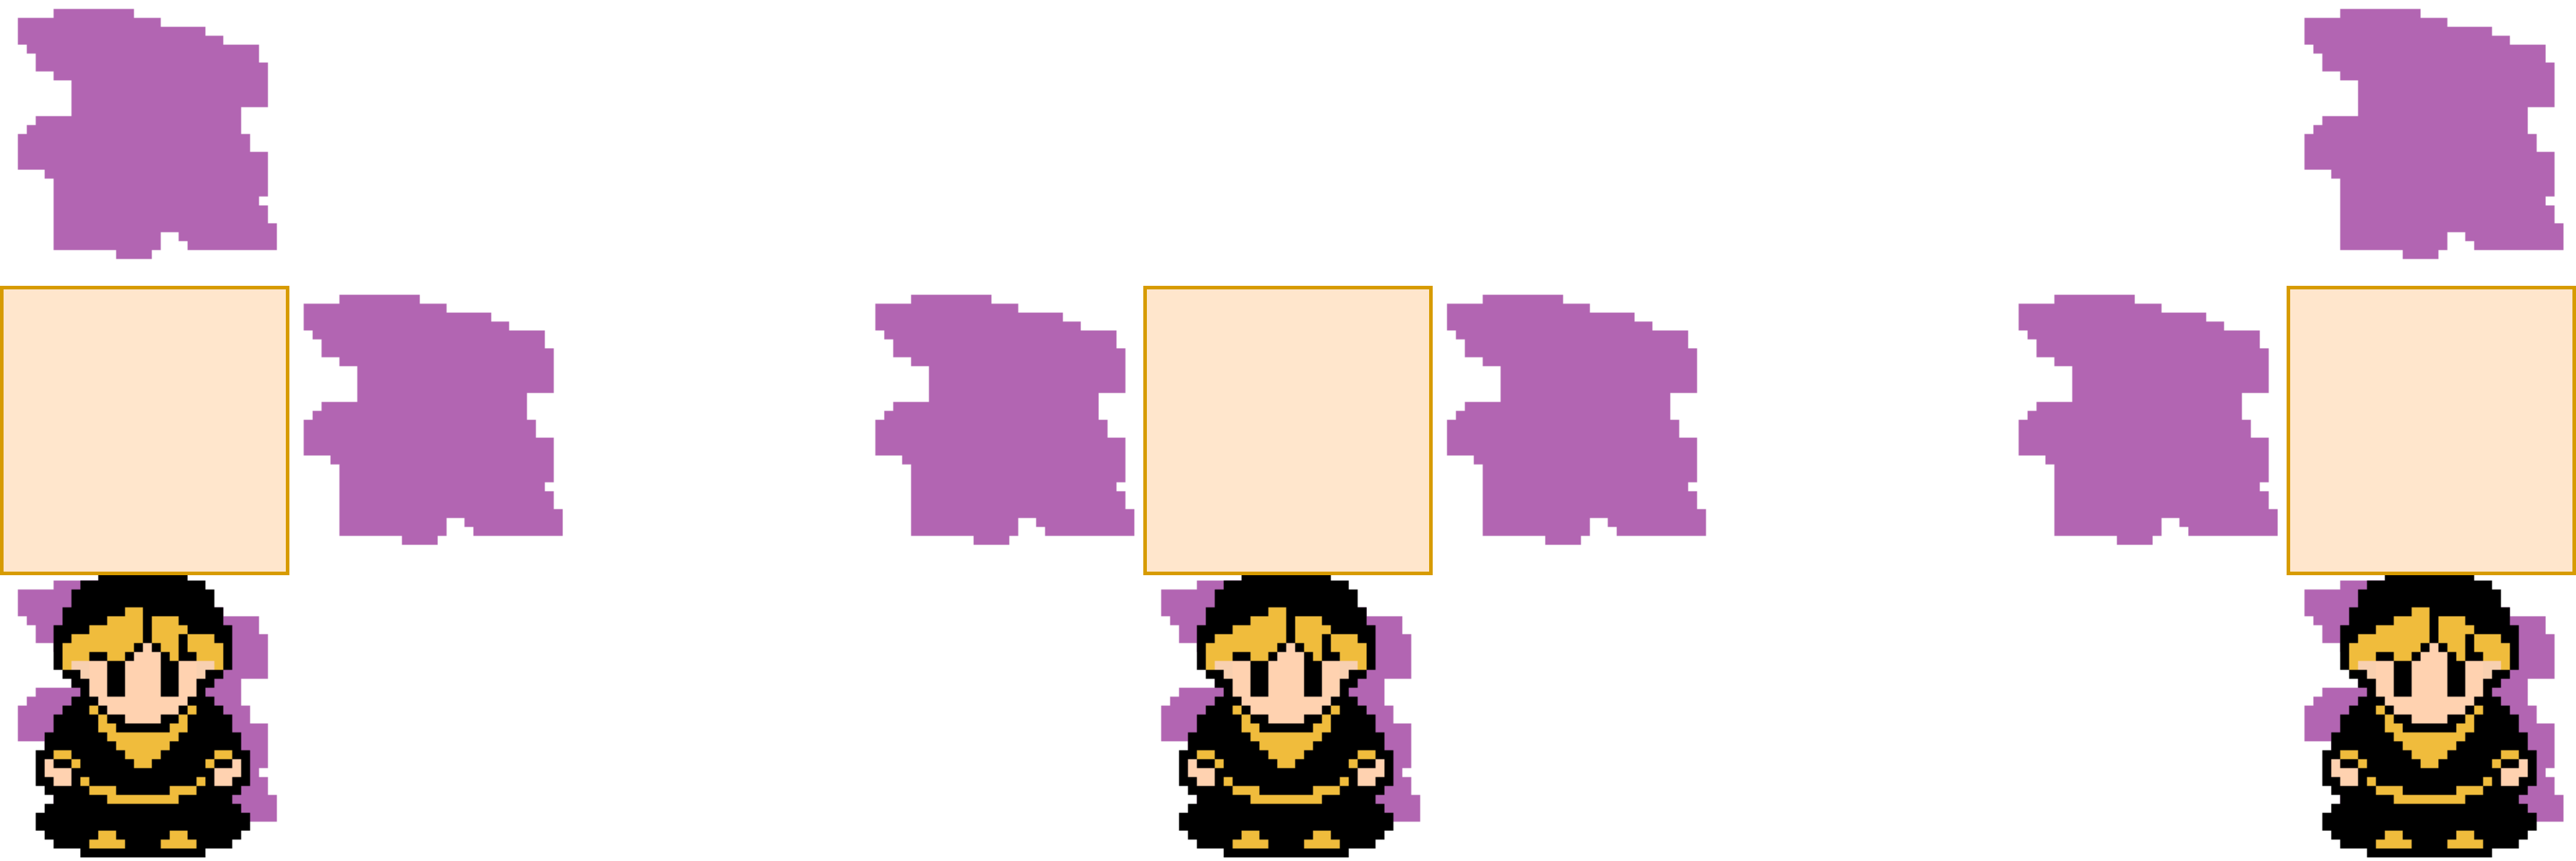
\includegraphics[width=.5\columnwidth]{w_norte}}\hspace{1em}
  \subfloat[W? al Este]{%
    
\includegraphics[width=.5\columnwidth]{w_este}}\\
  \subfloat[W? al Sur]{%
    
\includegraphics[width=.5\columnwidth]{w_sur}}\hspace{1em}
  \subfloat[W? al Oeste]{%
    
\includegraphics[width=.5\columnwidth]{w_oeste}}
  \caption{Inferir monstruo seguro}\label{fig:inferir_monstruo}
\end{figure}
\FloatBarrier

En caso de que no se haya percibido un hedor en la casilla en la que esta situado el agente, él sabe que las casillas adyacentes (\emph{Norte}, \emph{Este}, \emph{Sur} y \emph{Oeste}) es imposible que haya monstruos (los muros de la cueva no se pueden marcar como sin monstruo, ya que es incoherente hacerlo). Las reglas que permiten inferir esta conocimiento son:

\begin{itemize}
    \item $\neg H \land \neg M_{i, j-1} \longrightarrow OKW_{i, j-1}$
    \item $\neg H \land \neg M_{i+1, j} \longrightarrow OKW_{i+1, j}$
    \item $\neg H \land \neg M_{i, j+1} \longrightarrow OKW_{i, j+1}$
    \item $\neg H \land \neg M_{i-1, j1} \longrightarrow OKW_{i-1, j}$
\end{itemize}

\newpage
\centerline{\textbf{BRISA}}

La percepción de brisa indica que hay un posible precipicio cerca. El agente utiliza unas reglas similares a las de hedor para inferir sobre los precipicios (inferir posibles precipicios y precipicios seguros usando 3 brisas):

\begin{itemize}
    \item $B \land \neg M_{i, j-1} \land \neg W?_{i, j-1} \land \neg W_{i, j-1} \land \neg OKP_{i, j-1} \longrightarrow P?_{i, j-1}$
    \item $B \land \neg M_{i+1, j} \land \neg W?_{i+1, j} \land \neg W_{i+1, j} \land \neg OKP_{i+1, j} \longrightarrow P?_{i+1, j}$
    \item $B \land \neg M_{i, j+1} \land \neg W?_{i, j+1} \land \neg W_{i, j+1} \land \neg OKP_{i, j+1} \longrightarrow P?_{i, j+1}$
    \item $B \land \neg M_{i-1, j} \land \neg W?_{i-1, j} \land \neg W_{i-1, j} \land \neg OKP_{i-1, j} \longrightarrow P?_{i-1, j}$
\end{itemize}

\begin{itemize}
    \item Se ha percibido la brisa al SUR de un posible monstruo (Figura 3.2 (a)):
        \begin{itemize}
             \item $B \land P?_{i, j-1} \land B_{i+1, j-1} \land B_{i, j-2} \longrightarrow P_{i, j-1}$
             \item $B \land P?_{i, j-1} \land B_{i+1, j-1} \land B_{i-1, j-1} \longrightarrow P_{i, j-1}$
             \item $B \land P?_{i, j-1} \land B_{i-1, j-1} \land B_{i, j-2} \longrightarrow P_{i, j-1}$
        \end{itemize}
        
    \item Se ha percibido la brisa al OESTE de un posible monstruo (Figura 3.2 (b)):
        \begin{itemize}
            \item $B \land P?_{i+1, j} \land B_{i+1, j+1} \land B_{i+2, j} \longrightarrow P_{i+1, j}$
            \item $B \land P?_{i+1, j} \land B_{i+1, j+1} \land B_{i+1, j-1} \longrightarrow P_{i+1, j}$
            \item $B \land P?_{i+1, j} \land B_{i-1, j-1} \land B_{i+2, j} \longrightarrow P_{i+1, j}$
        \end{itemize}
        
    \item Se ha percibido la brisa al NORTE de un posible monstruo (Figura 3.2 (c)):
        \begin{itemize}
           \item $B \land P?_{i, j+1} \land B_{i-1, j+1} \land B_{i, j+2} \longrightarrow P_{i, j+1}$
            \item $B \land P?_{i, j+1} \land B_{i-1, j+1} \land B_{i+1, j+1} \longrightarrow P_{i, j+1}$
            \item $B \land P?_{i, j+1} \land B_{i+1, j+1} \land B_{i, j+2} \longrightarrow P_{i, j+1}$
        \end{itemize}
        
    \item Se ha percibido la brisa al ESTE de un posible monstruo (Figura 3.2 (d)):
        \begin{itemize}
            \item $B \land P?_{i-1, j} \land B_{i-1, j-1} \land B_{i-2, j} \longrightarrow P_{i-1, j+1}$
            \item $B \land P?_{i-1, j} \land B_{i-1, j-1} \land B_{i-1, j+1} \longrightarrow P_{i-1, j+1}$
            \item $B \land P?_{i-1, j} \land B_{i-1, j+1} \land B_{i-2, j} \longrightarrow P_{i-1, j+1}$
        \end{itemize}
\end{itemize}

\begin{figure}[htb]
\centering
  \subfloat[P? al Norte]{%
    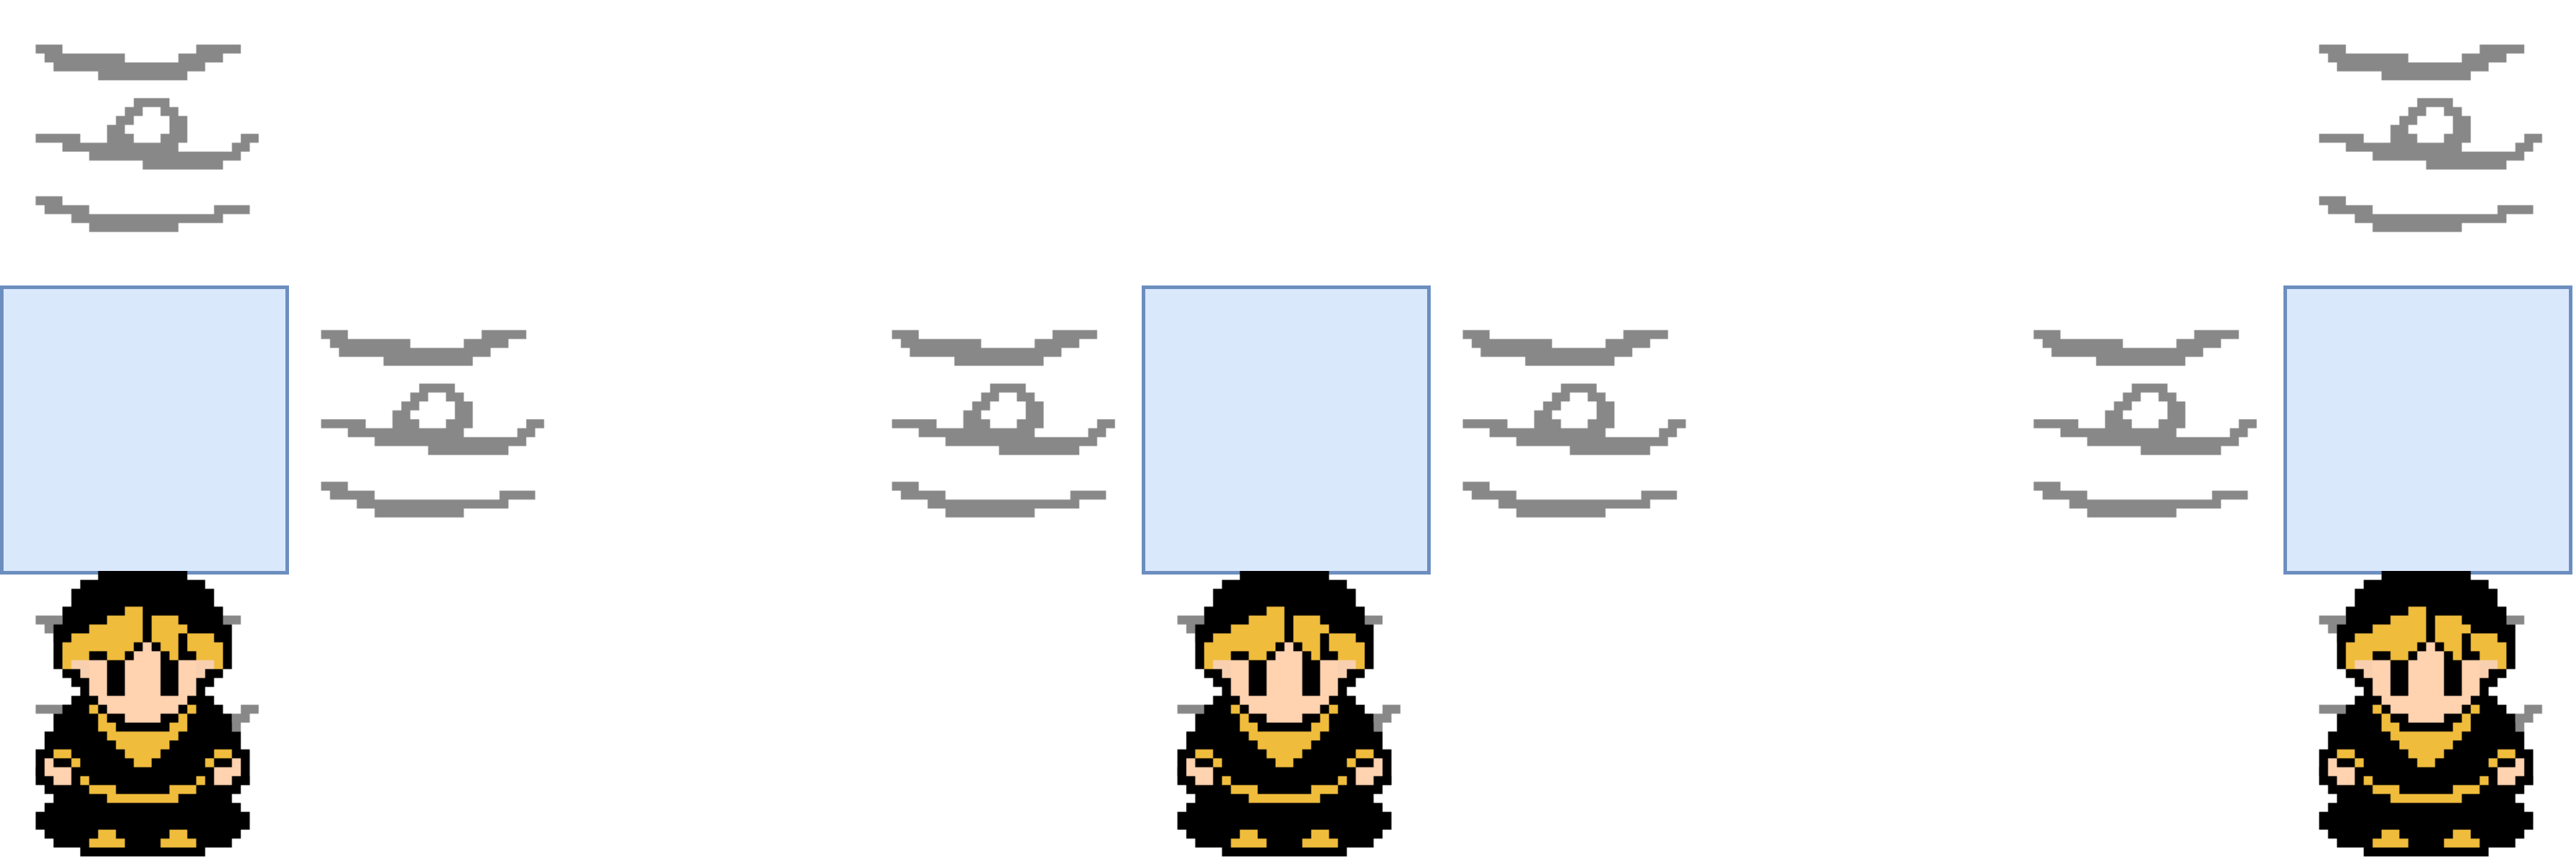
\includegraphics[width=.5\columnwidth]{p_norte}}\hspace{1em}
  \subfloat[P? al Este]{%
    
\includegraphics[width=.5\columnwidth]{p_este}}\\
  \subfloat[P? al Sur]{%
    
\includegraphics[width=.5\columnwidth]{p_sur}}\hspace{1em}
  \subfloat[P? al Oeste]{%
    
\includegraphics[width=.5\columnwidth]{p_oeste}}
  \caption{Inferir precipicio seguro}\label{fig:inferir_precipicio}
\end{figure}
\FloatBarrier

\begin{itemize}
    \item $\neg B \land \neg M_{i, j-1} \longrightarrow OKP_{i, j-1}$
    \item $\neg B \land \neg M_{i+1, j} \longrightarrow OKP_{i+1, j}$
    \item $\neg B \land \neg M_{i, j+1} \longrightarrow OKP_{i, j+1}$
    \item $\neg B \land \neg M_{i-1, j1} \longrightarrow OKP_{i-1, j}$
\end{itemize}

\centerline{\textbf{INCREMENTAR CASILLAS SEGURAS SIN CONSUMIR}}

Se incrementa el contador de casillas seguras conocidas sin visitar en función del número de casillas seguras adyacentes sin visitar y se las marca como sin consumir.

\begin{itemize}
    \item $OK_{i, j-1} \wedge \neg V_{i,j-1} \wedge \neg SC_{i, j-1} \longrightarrow SC := SC + 1, SC_{i,j-1}$
    \item $OK_{i+1, j} \wedge \neg V_{i+1,j} \wedge \neg SC_{i+1, j} \longrightarrow SC := SC + 1, SC_{i+1,j}$
    \item $OK_{i, j+1} \wedge \neg V_{i,j+1} \wedge \neg SC_{i, j+1} \longrightarrow SC := SC + 1, SC_{i,j+1}$
    \item $OK_{i-1, j} \wedge \neg V_{i-1,j} \wedge \neg SC_{i-1, j} \longrightarrow SC := SC + 1, SC_{i-1,j}$
\end{itemize}

\section{Parte reactiva}

En la parte reactiva de las reglas que permiten realizar acciones correctas y seguras con el conocimiento inferido en la base de conocimientos. Estas reglas son:

\begin{itemize}
    \item Recoger el tesoro en una casillas con resplandor.
        \begin{itemize}
            \item   $X_1 \longrightarrow RECOGER\_TESORO \equiv$
                    \newline
                    $T_{i, j} \longrightarrow RECOGER\_TESORO$
        \end{itemize}
        
    \item Lanzar bombas de hedor cuando el tiempo de espera (aleatorio) ha terminado.
        \begin{itemize}
            \item $X_2 \longrightarrow PRODUCIR\_HEDOR$
            \newline
            $CR = 0 \land BR > 0 \longrightarrow PRODUCIR\_HEDOR$
        \end{itemize}
    
    \item Matar el monstruo seguro (se prefiere a visitar casillas adyacentes que la muerte de un monstruo puede suponer la posibilidad de explorar más la cueva y encontrar el tesoro): 
        \begin{itemize}
            \item   $X_3 \longrightarrow DISPARAR\_NORTE \equiv$
                    \newline
                    $W_{i, j-1} \land PR > 0 \longrightarrow DISPARAR\_NORTE$
            \item   $X_4 \longrightarrow DISPARAR\_ESTE \equiv$
                    \newline
                    $W_{i+1, j} \land PR > 0 \longrightarrow DISPARAR\_ESTE$
            \item   $X_5 \longrightarrow DISPARAR\_SUR \equiv$
                    \newline
                    $W_{i, j+1} \land PR > 0 \longrightarrow DISPARAR\_SUR$
            \item   $X_6 \longrightarrow DISPARAR\_OESTE \equiv$
                    \newline
                    $W_{i-1, j} \land PR > 0 \longrightarrow DISPARAR\_OESTE$
        \end{itemize}
    
    \item Explorar casillas no visitadas y que sean seguras:
        \begin{itemize}
            \item   $ X_7                 \longrightarrow$
                    $A = DESPLAZARSE\_NORTE $
                    $\equiv$
                    \newline
                    $ A = NINGUNA \land \neg M_{i, j-1} \land \neg V_{i, j-1} \land OK_{i, j-1} \longrightarrow$
                    \newline
                    $A = DESPLAZARSE\_NORTE$
            
             \item  $ X_8                 \longrightarrow$
                    $A = DESPLAZARSE\_ESTE $
                    $\equiv$
                    \newline
                    $ A = NINGUNA \land \neg M_{i+1, j} \land \neg V_{i+1, j} \land OK_{i+1, j} \longrightarrow$
                    \newline
                    $A = DESPLAZARSE\_ESTE $
                    
             \item  $ X_9                 \longrightarrow$
                    $A = DESPLAZARSE\_SUR $
                    $\equiv$
                    \newline
                    $ A = NINGUNA \land \neg M_{i, j+1} \land \neg V_{i, +1j} \land OK_{i, j+1} \longrightarrow$
                    \newline
                    $A = DESPLAZARSE\_SUR $
            
             \item  $ X_{10}                 \longrightarrow$
                    $A = DESPLAZARSE\_OESTE $
                    $\equiv$
                    \newline
                    $ A = NINGUNA \land \neg M_{i-1, j} \land \neg V_{i-1, j} \land OK_{i-1, j} \longrightarrow$
                    \newline
                    $A = DESPLAZARSE\_OESTE $
            
        \end{itemize}
    
    \item Realizar un disparo en caso de que existan posibles monstruos y el agente no tenga más casillas por explorar:
        \begin{itemize}
            \item $X_{11} \longrightarrow DISPARAR\_NORTE$
            $\equiv$
            \newline
            $A = NINGUNA \land SC = 0 \land W?_{i, j-1} \land PR > 0$ 
            
            $\longrightarrow DISPARAR\_NORTE$
            
            \item $X_{12} \longrightarrow DISPARAR\_ESTE$
            $\equiv$
            \newline
            $A = NINGUNA \land SC = 0 \land W?_{i+1, j} \land PR > 0$ 
            
            $\longrightarrow DISPARAR\_ESTE$
            
            \item $X_{13} \longrightarrow DISPARAR\_SUR$
            $\equiv$
            \newline
            $A = NINGUNA \land SC = 0 \land W?_{i, j+1} \land PR > 0$ 
            
            $\longrightarrow DISPARAR\_SUR$
            
            \item $X_{14} \longrightarrow DISPARAR\_OESTE$
            $\equiv$
            \newline
            $A = NINGUNA \land SC = 0 \land W?_{i-1, j} \land PR > 0$ 
            
            $\longrightarrow DISPARAR\_OESTE$
        \end{itemize}
    
    \item Volver a la casilla anterior (realizar la acción contraria) en caso de que no se haya podido cumplir ninguno de los casos anteriores:
        \begin{itemize}
            \item $A = NINGUNA \longrightarrow VOLVER\_CASILLA\_ANTERIOR$
        \end{itemize}
\end{itemize}

\newpage
\section{Todas las reglas}

Finalmente, el conjunto de todas las reglas es:
\begin{enumerate}
    \item $\neg V_{i, j} \longrightarrow SC := SC - 1$
    \item $1 \longrightarrow V_{i, j}$
    \item $V_{i, j} \longrightarrow OK_{i, j}$
    \item $OK_{i, j} \iff OKW_{i, j} \land OKP_{i, j} $
    \item $OKW_{i, j} \longrightarrow \neg W?_{i, j} \land \neg W_{i, j} $
    \item $OKP_{i, j} \longrightarrow \neg P?_{i, j} \land \neg P_{i, j} $
    \item $P_{i, j} \longrightarrow \neg P?_{i, j} \land \neg W?_{i, j} \land \neg W_{i, j}$
    \item $W_{i, j} \longrightarrow \neg W?_{i, j} \land \neg P?_{i, j} \land \neg P_{i, j}$
    \item $W_{i, j} \longrightarrow \neg V_{i, j}$
    \item $ S \land A^{t-1} = DISPARAR\_NORTE \longrightarrow OKW_{i, j-1} $
    \item $ S \land A^{t-1} = DISPARAR\_ESTE \longrightarrow OKW_{i+1, j} $
    \item $ S \land A^{t-1} = DISPARAR\_SUR \longrightarrow OKW_{i, j+1} $
    \item $ S \land A^{t-1} = DISPARAR\_OESTE \longrightarrow OKW_{i-1, j} $
    \item $ \neg S \land A^{t-1} = DISPARAR\_NORTE \longrightarrow OKW_{i, j-1} \land ... \land OKW_{i, 0} $
    \item $ \neg S \land A^{t-1} = DISPARAR\_ESTE \longrightarrow OKW_{i+1, j} \land ... \land OKW_{n-1, j}$
    \item $ \neg S \land A^{t-1} = DISPARAR\_SUR \longrightarrow OKW_{i, j+1}  \land ... \land OKW_{i, m-1}$
    \item $ \neg S \land A^{t-1} = DISPARAR\_OESTE \longrightarrow OKW_{i-1, j} \land ... \land OKW_{0, j}$ 
    \item $R_{i, j} \longrightarrow T_{i, j}$
    \item $\neg R_{i, j} \longrightarrow \neg T_{i, j}$
    \item $G \land A^{t-1} = DESPLAZARSE\_NORTE \longrightarrow M_{0, j-1} \land ... \land M_{n, j-1}$
    \item $G \land A^{t-1} = DESPLAZARSE\_NORTE \land SC_{0, j-1} \longrightarrow SC := SC - 1,$ \newline
    $G \land A^{t-1} = DESPLAZARSE\_NORTE \land SC_{1, j-1} \longrightarrow SC := SC - 1,$ \newline
    $...,$ \newline
    $G \land A^{t-1} = DESPLAZARSE\_NORTE \land SC_{n, j-1} \longrightarrow SC := SC - 1$
    \item $G \land A^{t-1} = DESPLAZARSE\_ESTE \longrightarrow M_{i+1, 0} \land ... \land M_{i+1, m}$
    \item $G \land A^{t-1} = DESPLAZARSE\_ESTE \land SC_{i+1, 0} \longrightarrow SC := SC - 1,$ \newline
    $G \land A^{t-1} = DESPLAZARSE\_ESTE \land SC_{i+1, 1} \longrightarrow SC := SC - 1,$ \newline
    $...,$ \newline
    $G \land A^{t-1} = DESPLAZARSE\_ESTE \land SC_{i+1,m} \longrightarrow SC := SC - 1$
    \item $G \land A^{t-1} = DESPLAZARSE\_SUR \longrightarrow M_{0, j+1} \land ... \land M_{n, j+1}$
    \item $G \land A^{t-1} = DESPLAZARSE\_SUR \land SC_{0, j+1} \longrightarrow SC := SC - 1,$ \newline
    $G \land A^{t-1} = DESPLAZARSE\_SUR \land SC_{1, j+1} \longrightarrow SC := SC - 1,$ \newline
    $...,$ \newline
    $G \land A^{t-1} = DESPLAZARSE\_SUR \land SC_{n, j+1} \longrightarrow SC := SC - 1$
    \item $G \land A^{t-1} = DESPLAZARSE\_OESTE \longrightarrow M_{i-1, 0} \land ... \land M_{i-1, m}$
    \item $G \land A^{t-1} = DESPLAZARSE\_OESTE \land SC_{i-1, 0} \longrightarrow SC := SC - 1,$ \newline
    $G \land A^{t-1} = DESPLAZARSE\_OESTE \land SC_{i-1, 1} \longrightarrow SC := SC - 1,$ \newline
    $...,$ \newline
    $G \land A^{t-1} = DESPLAZARSE\_OESTE \land SC_{i-1,m} \longrightarrow SC := SC - 1$
    \item $H \land \neg M_{i, j-1} \land \neg P?_{i, j-1} \land \neg P_{i, j-1} \land \neg OKW_{i, j-1} \longrightarrow W?_{i, j-1}$
    \item $H \land \neg M_{i+1, j} \land \neg P?_{i+1, j} \land \neg P_{i+1, j} \land \neg OKW_{i+1, j} \longrightarrow W?_{i+1, j}$
    \item $H \land \neg M_{i, j+1} \land \neg P?_{i, j+1} \land \neg P_{i, j+1} \land \neg OKW_{i, j+1} \longrightarrow W?_{i, j+1}$
    \item $H \land \neg M_{i-1, j} \land \neg P?_{i-1, j} \land \neg P_{i-1, j} \land \neg OKW_{i-1, j} \longrightarrow W?_{i-1, j}$
    \item $H \land W?_{i, j-1} \land H_{i+1, j-1} \land H_{i, j-2} \longrightarrow W_{i, j-1}$
    \item $H \land W?_{i, j-1} \land H_{i+1, j-1} \land H_{i-1, j-1} \longrightarrow W_{i, j-1}$
    \item $H \land W?_{i, j-1} \land H_{i-1, j-1} \land H_{i, j-2} \longrightarrow W_{i, j-1}$
    
    \item $H \land W?_{i+1, j} \land H_{i+1, j+1} \land H_{i+2, j} \longrightarrow W_{i+1, j}$
    \item $H \land W?_{i+1, j} \land H_{i+1, j+1} \land H_{i+1, j-1} \longrightarrow W_{i+1, j}$
    \item $H \land W?_{i+1, j} \land H_{i-1, j-1} \land H_{i+2, j} \longrightarrow W_{i+1, j}$
    
    \item $H \land W?_{i, j+1} \land H_{i-1, j+1} \land H_{i, j+2} \longrightarrow W_{i, j+1}$
    \item $H \land W?_{i, j+1} \land H_{i-1, j+1} \land H_{i+1, j+1} \longrightarrow W_{i, j+1}$
    \item $H \land W?_{i, j+1} \land H_{i+1, j+1} \land H_{i, j+2} \longrightarrow W_{i, j+1}$
    
    \item $H \land W?_{i-1, j} \land H_{i-1, j-1} \land H_{i-2, j} \longrightarrow W_{i-1, j+1}$
    \item $H \land W?_{i-1, j} \land H_{i-1, j-1} \land H_{i-1, j+1} \longrightarrow W_{i-1, j+1}$
    \item $H \land W?_{i-1, j} \land H_{i-1, j+1} \land H_{i-2, j} \longrightarrow W_{i-1, j+1}$
    
    \item $B \land \neg M_{i, j-1} \land \neg W?_{i, j-1} \land \neg W_{i, j-1} \land \neg OKP_{i, j-1} \longrightarrow P?_{i, j-1}$
    \item $B \land \neg M_{i+1, j} \land \neg W?_{i+1, j} \land \neg W_{i+1, j} \land \neg OKP_{i+1, j} \longrightarrow P?_{i+1, j}$
    \item $B \land \neg M_{i, j+1} \land \neg W?_{i, j+1} \land \neg W_{i, j+1} \land \neg OKP_{i, j+1} \longrightarrow P?_{i, j+1}$
    \item $B \land \neg M_{i-1, j} \land \neg W?_{i-1, j} \land \neg W_{i-1, j} \land \neg OKP_{i-1, j} \longrightarrow P?_{i-1, j}$
    \item $B \land P?_{i, j-1} \land B_{i+1, j-1} \land B_{i, j-2} \longrightarrow P_{i, j-1}$
    \item $B \land P?_{i, j-1} \land B_{i+1, j-1} \land B_{i-1, j-1} \longrightarrow P_{i, j-1}$
    \item $B \land P?_{i, j-1} \land B_{i-1, j-1} \land B_{i, j-2} \longrightarrow P_{i, j-1}$
    
    \item $B \land P?_{i+1, j} \land B_{i+1, j+1} \land B_{i+2, j} \longrightarrow P_{i+1, j}$
    \item $B \land P?_{i+1, j} \land B_{i+1, j+1} \land B_{i+1, j-1} \longrightarrow P_{i+1, j}$
    \item $B \land P?_{i+1, j} \land B_{i-1, j-1} \land B_{i+2, j} \longrightarrow P_{i+1, j}$
    
    \item $B \land P?_{i, j+1} \land B_{i-1, j+1} \land B_{i, j+2} \longrightarrow P_{i, j+1}$
    \item $B \land P?_{i, j+1} \land B_{i-1, j+1} \land B_{i+1, j+1} \longrightarrow P_{i, j+1}$
    \item $B \land P?_{i, j+1} \land B_{i+1, j+1} \land B_{i, j+2} \longrightarrow P_{i, j+1}$
    
    \item $B \land P?_{i-1, j} \land B_{i-1, j-1} \land B_{i-2, j} \longrightarrow P_{i-1, j+1}$
    \item $B \land P?_{i-1, j} \land B_{i-1, j-1} \land B_{i-1, j+1} \longrightarrow P_{i-1, j+1}$
    \item $B \land P?_{i-1, j} \land B_{i-1, j+1} \land B_{i-2, j} \longrightarrow P_{i-1, j+1}$
    
    \item $OK_{i, j-1} \wedge \neg V_{i,j-1} \wedge \neg SC_{i, j-1} \longrightarrow SC := SC + 1, SC_{i,j-1}$
    \item $OK_{i+1, j} \wedge \neg V_{i+1,j} \wedge \neg SC_{i+1, j} \longrightarrow SC := SC + 1, SC_{i+1,j}$
    \item $OK_{i, j+1} \wedge \neg V_{i,j+1} \wedge \neg SC_{i, j+1} \longrightarrow SC := SC + 1, SC_{i,j+1}$
    \item $OK_{i-1, j} \wedge \neg V_{i-1,j} \wedge \neg SC_{i-1, j} \longrightarrow SC := SC + 1, SC_{i-1,j}$
\newline
    \item   $X_1 \longrightarrow RECOGER\_TESORO \equiv$
    \newline
    $T_{i, j} \longrightarrow RECOGER\_TESORO$

    \item $X_2 \longrightarrow PRODUCIR\_HEDOR$
    \newline
    $CR = 0 \land BR > 0 \longrightarrow PRODUCIR\_HEDOR$

    \item   $X_3 \longrightarrow DISPARAR\_NORTE \equiv$
    \newline
    $W_{i, j-1} \land PR > 0 \longrightarrow DISPARAR\_NORTE$

    \item   $X_4 \longrightarrow DISPARAR\_ESTE \equiv$
    \newline
    $W_{i+1, j} \land PR > 0 \longrightarrow DISPARAR\_ESTE$

    \item   $X_5 \longrightarrow DISPARAR\_SUR \equiv$
    \newline
    $W_{i, j+1} \land PR > 0 \longrightarrow DISPARAR\_SUR$

    \item   $X_6 \longrightarrow DISPARAR\_OESTE \equiv$
    \newline
    $W_{i-1, j} \land PR > 0 \longrightarrow DISPARAR\_OESTE$

    \item   $ X_7                 \longrightarrow$
    $A = DESPLAZARSE\_NORTE $
    $\equiv$
    \newline
    $ A = NINGUNA \land \neg M_{i, j-1} \land \neg V_{i, j-1} \land OK_{i, j-1} \longrightarrow$
    \newline
    $A = DESPLAZARSE\_NORTE$
            
    \item  $ X_8                 \longrightarrow$
    $A = DESPLAZARSE\_ESTE $
    $\equiv$
    \newline
    $ A = NINGUNA \land \neg M_{i+1, j} \land \neg V_{i+1, j} \land OK_{i+1, j} \longrightarrow$
    \newline
    $A = DESPLAZARSE\_ESTE $
                    
    \item  $ X_9                 \longrightarrow$
    $A = DESPLAZARSE\_SUR $
    $\equiv$
    \newline
    $ A = NINGUNA \land \neg M_{i, j+1} \land \neg V_{i, +1j} \land OK_{i, j+1} \longrightarrow$
    \newline
    $A = DESPLAZARSE\_SUR $
            
    \item  $ X_{10}                 \longrightarrow$
    $A = DESPLAZARSE\_OESTE $
    $\equiv$
    \newline
    $ A = NINGUNA \land \neg M_{i-1, j} \land \neg V_{i-1, j} \land OK_{i-1, j} \longrightarrow$
    \newline
    $A = DESPLAZARSE\_OESTE $

    \item $X_{11} \longrightarrow DISPARAR\_NORTE$
    $\equiv$
    \newline
    $A = NINGUNA \land SC = 0 \land W?_{i, j-1} \land PR > 0$ 
            
    $\longrightarrow DISPARAR\_NORTE$
            
    \item $X_{12} \longrightarrow DISPARAR\_ESTE$
    $\equiv$
    \newline
    $A = NINGUNA \land SC = 0 \land W?_{i+1, j} \land PR > 0$ 
            
    $\longrightarrow DISPARAR\_ESTE$
            
    \item $X_{13} \longrightarrow DISPARAR\_SUR$
    $\equiv$
    \newline
    $A = NINGUNA \land SC = 0 \land W?_{i, j+1} \land PR > 0$ 
            
    $\longrightarrow DISPARAR\_SUR$
            
    \item $X_{14} \longrightarrow DISPARAR\_OESTE$
    $\equiv$
    \newline
    $A = NINGUNA \land SC = 0 \land W?_{i-1, j} \land PR > 0$ 
            
    $\longrightarrow DISPARAR\_OESTE$

    \item $A = NINGUNA \longrightarrow VOLVER\_CASILLA\_ANTERIOR$
\end{enumerate}{}

\end{document}
